\documentclass[a2paper, 12pt]{article}
\usepackage[font={huge, bf}]{caption}
\usepackage{fontspec}
\setmainfont{Arial}
\usepackage{subcaption}
\usepackage{graphicx}
\usepackage{tikz}
\usepackage{tikzsymbols}
\usetikzlibrary{calc,patterns,shapes.geometric}
\usepackage{float}
\usepackage{pdflscape}
\usepackage{geometry}
\geometry{landscape, margin=2cm}
\captionsetup[subfigure]{justification=justified,singlelinecheck=false}
\pagestyle{empty}

\def\centerarc[#1](#2)(#3:#4:#5){\draw[#1] ($(#2)+({#5*cos(#3)},{#5*sin(#3)})$) arc (#3:#4:#5);}

\begin{document}
	\vspace*{\fill}
	\begin{figure}[!htbp]
		\centering
		\begin{subfigure}[b]{0.48\textwidth}
			\caption{Figure 1}
			\centering
			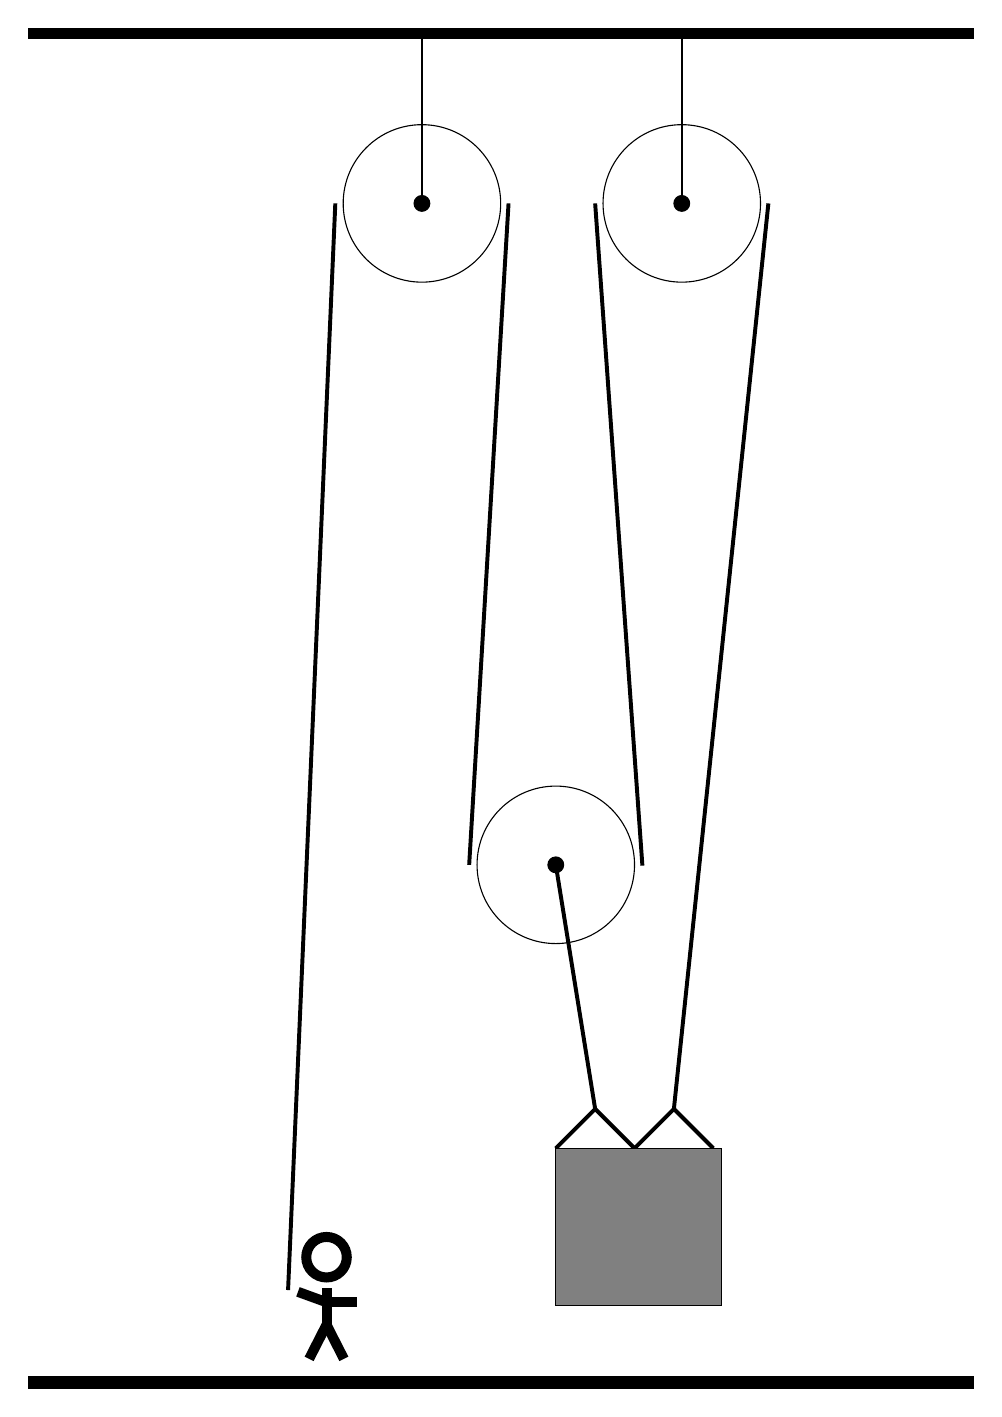
\begin{tikzpicture}
				\draw[fill=black] (-4, 14) rectangle (8, 14.125);
				
				\draw (1, 11.9) circle (1);
				\draw[fill=black] (1, 11.9) circle (0.1);
				\draw[thick] (1, 11.9) -- (1, 14);
				
				\draw (4.3, 11.9) circle (1);
				\draw[fill=black] (4.3, 11.9) circle (0.1);
				\draw[thick] (4.3, 11.9) -- (4.3, 14);
				
				\draw (2.7, 3.5) circle (1);
				\draw[fill=black] (2.7, 3.5) circle (0.1);
				
				\draw[line width=0.5mm]  (2.7, -0.1) -- (3.2, 0.4) -- (3.7, -0.1) -- (4.2, 0.4) -- (4.7, -0.1);
				\draw[fill=black!50] (2.7, -0.1) rectangle (4.8, -2.1);
				
				\draw[line width=0.5mm](-0.7, -1.9) -- (-0.1, 11.9);
				\centerarc[line width=0.5mm](1, 11.9)(0:180:1.1);
				\draw[line width=0.5mm](2.1, 11.9) -- (1.6, 3.5);
				\centerarc[line width=0.5mm](2.7, 3.5)(180:370:1.1);
				\draw[line width=0.5mm] (3.8, 3.49) -- (3.2, 11.9);
				\centerarc[line width=0.5mm](4.3, 11.9)(0:180:1.1);
				\draw[line width=0.5mm](4.2, 0.4) -- (5.4, 11.9);
				\draw[line width=0.5mm] (3.2, 0.4) -- (2.7, 3.5);
				
				\node at (-0.2, -2) {\scriptsize \Strichmaxerl[10][-20][0]};
				
				\draw[fill=black] (-4, -3) rectangle (8, -3.15);
			\end{tikzpicture}
		\end{subfigure}
		\hfill
		\begin{subfigure}[b]{0.48\textwidth}
			\caption{Figure 2}
			\centering
			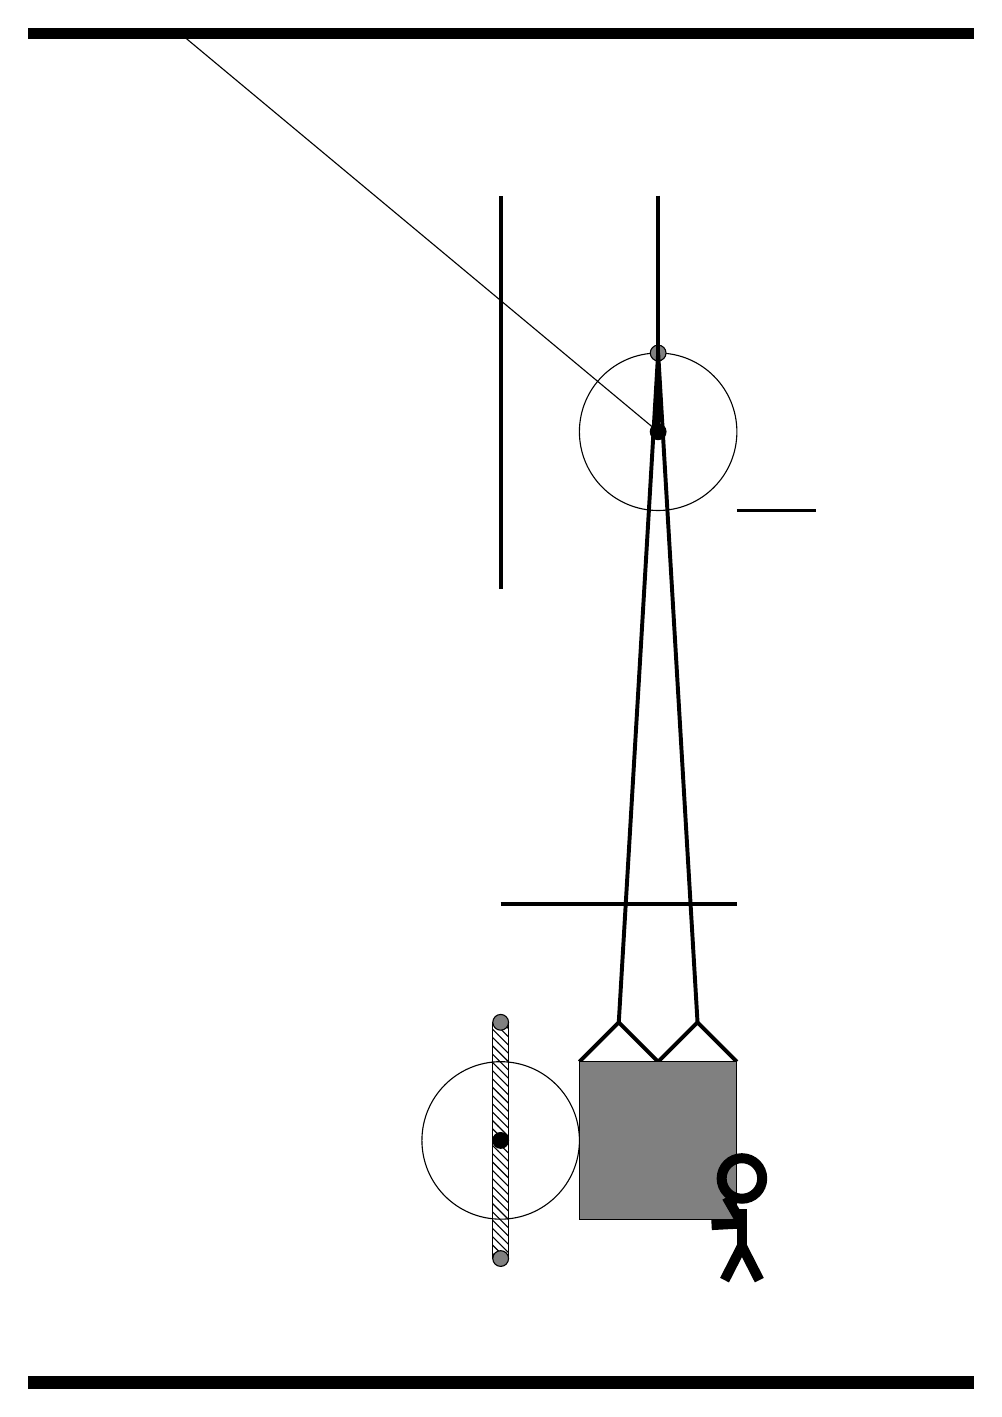
\begin{tikzpicture}
				\draw[fill=black] (-4, 14) rectangle (8, 14.125);
				
				\draw (4,9) circle (1);
				\draw[fill=black] (4,9) circle (0.1);
				\draw (-2,14.0) -- (4,9);
				
				\draw (2,0) circle (1);
				\draw[fill=black] (2,0) circle (0.1);
				\draw[pattern=north west lines, pattern color=black] (1.9,1.5) rectangle (2.1,-1.5);
				\draw[fill=black!50] (2,1.5) circle (0.1);
				\draw[fill=black!50] (2,-1.5) circle (0.1);
				
				\draw[fill=black!50] (4,10) circle (0.1);
				\draw[line width=0.5mm](3.5,1.5) -- (4,10) --  (4.5,1.5);
				\draw[line width=0.5mm](3,1) --  (3.5,1.5) -- (4,1) -- (4.5,1.5) -- (5,1);
				\draw[fill=black!50] (3, 1) rectangle (5, -1);
				
				\draw[line width = 0.5mm] (2,7) -- (2,12);
				\centerarc[line width = 0.5mm](3,12)(0:180:1);
				\draw[line width = 0.5mm] (4,12) -- (4,9);
				\centerarc[line width = 0.5mm](5,9)(270:180:1);
				\draw[line width = 0.5mm] (5,8) -- (6,8);
				\draw[line width = 0.5mm] (2,3) -- (5,3);
				\centerarc[line width = 0.5mm](2,2)(90:180:1);
				
				\node at (5, -1) {\scriptsize \Strichmaxerl[10][3][120]};
				
				\draw[fill=black] (-4, -3) rectangle (8, -3.15);
			\end{tikzpicture}
		\end{subfigure}
	\end{figure}
		\vspace*{\fill}
\end{document}